
\section{Nuclear Decay and Radiocarbon Dating}

Name \rule{2.0in}{0.1pt}\hfill{}Section \rule{1.0in}{0.1pt}\hfill{}Date
\rule{1.0in}{0.1pt}

\textbf{Objective}

To develop an understanding of the use of the radioactive decay of
atomic nuclei to date objects like the Shroud of Turin.

\textbf{Apparatus}

\begin{itemize}

\item Radioactive sources.
\item Radiation counter.
\item Jack.
\item Isotope generator.
\item Surgical gloves, eye protection, and lab coat for handling radioactive liquids.
\item Lead and plastic sheets.

\end{itemize}

\textbf{Introduction}

Atoms can be broken down into light, negatively-charged, electrons,
and a small, dense, positively-charged nucleus. These atomic nuclei
can spontaneously break apart into smaller nuclei in a process called
radioactive decay. By measuring the rate of this decay under the appropriate
circumstances one can develop a {}``clock'' that can be used to
determine how long ago in the past an event occurred. In this laboratory
we will apply this notion to a particular object, the Shroud of Turin
which is purported to be the burial cloth of Jesus Christ.

\textbf{Activity 1: Nuclear Terminology }

Atomic nuclei can be constructed from protons and neutrons. The number
of protons in a nucleus is called the atomic number and is represented
by the letter Z while the number of neutrons is represented by the
letter N. The protons carry a charge of +e while the neutrons are
electrically neutral. The sum of these two quantities is the mass
number A.

{\centering A = N + Z\par}

Protons and neutrons are often referred to as nucleons.

Nuclei are represented using their chemical symbol (determined by
the atomic number) and the mass number. For example, the most common
form of carbon has six protons and six neutrons in its nucleus and
is written as \( ^{12} \)C. If another neutron is added to this nucleus,
then one has an isotope of carbon, \( ^{13} \)C. Isotopes of a chemical element
have the same atomic number(Z), but have a different numbers of neutrons
(N) and a different mass number (A). The difference is reflected in
the value of the superscript on the chemical symbol.

(a) Consider the following list of the number of protons and neutrons
that combine to form a particular nucleus. In the third column enter the chemical
symbol and mass number as shown above (e.g., \( ^{12} \)C). Use the
periodic chart at the end of this unit to determine what to enter in the third
column.

\vspace{0.3cm}
{\centering \begin{tabular}{|c|c|c|}
\hline 
Number of Protons&
Number of Neutrons&
Nucleus\\
\hline
\hline 
7&
8&
\\
\hline 
79&
118&
\\
\hline 
26&
30&
\\
\hline
\end{tabular}\par}
\vspace{0.3cm}

(b) Consider the following list of atomic nuclei. In the second and
third columns enter the number of protons and neutrons in each nucleus.

\vspace{0.3cm}
{\centering \begin{tabular}{|c|c|c|}
\hline 
Nucleus&
Number of Protons&
Number of Neutrons\\
\hline
\hline 
\( ^{4} \)He&
&
\\
\hline 
\( ^{235} \)U&
&
\\
\hline 
\( ^{108} \)Ag&
&
\\
\hline
\end{tabular}\par}
\vspace{0.3cm}

Some isotopes can spontaneously decay into other nuclei.
In many of these decays the number of nucleons is conserved. 
This
means that the number of protons and neutrons added together in the parent nucleus before
the decay must be the same in the final products.
Electric charge
is always conserved.

(c) In the table below a nuclear decay is shown in the first column.
In most cases the original nucleus (often referred to as the parent)
produces two smaller nuclei (called daughters). Only one of the
daughter nuclei is listed. In the adjacent column list the missing
nucleus.
Notice there are two emitted particles that we have not mentioned
before.
The $e^-$ which is an electron and is often called a
beta particle.
It has almost zero mass compared to a nucleon.
The other is $\gamma$ and is called a ``gamma'' particle.
This is photon or a particle of light
or electromagnetic energy.
The gamma has no mass or charge, but does carry energy and momentum.

\vspace{0.3cm}
{\centering \begin{tabular}{|c|c|}
\hline 
~~~~~~~~~~~~~Decay~~~~~~~~~~~~~&
~~~~~~~~Unknown~~~~~~~~\\
\hline
\hline 
\( ^{190} \)Po \( \rightarrow  \) \( ^{4} \)He + ?&
\\
\hline 
\( ^{210} \)Th \( \rightarrow  \) \( ^{4} \)He + ?&
\\
\hline 
\( ^{16} \)Ne \( \rightarrow  \) p + ?&
\\
\hline 
\( ^{90} \)Sr \( \rightarrow  \) \(e^-\) + ?&
\\
\hline 
\( ^{60} \)Co \( \rightarrow  \) \(\gamma\) + ?&
\\
\hline
\end{tabular}\par}
\vspace{0.3cm}

% \textbf{Activity 2: Calibrating the Geiger Counter} 

%Before we proceed we have to understand how to use the device that will detect
%the radiation from radioactive material.
%The device is called a Geiger counter and it will ``count'' the number
%of nuclear particles that pass through it.
%The device consists of a sealed cylinder with a wire
%running down the center and argon gas filling the cylinder.
%The center wire is kept at a large, positive voltage while the walls of the cylinder
%are at zero or negative voltage.
%When an energetic nuclear particle passes through the counter it ionizes the argon
%atoms in the cylinder.
%The electrons are attracted to the center wire and produce a voltage pulse which is
%detected and counted by the electronics. 
%To count the number of particles that pass through the detector accurately
%the voltage of the center wire must be set to produce the same signal regardless of the energy
%of the particle passing through the Geiger tube.
%To find this ``plateau'' voltage follow the procedure below.

%(a) Make sure the Geiger counter is plugged into the computer interface and into the power
%supply. If not, consult your instructor.

%(b) There will be a radioactive source at each station for calibrating the Geiger counter.
%The window on the end of the cylinder is very fragile so avoid touching it at all costs.
%Place the radioactive source on the square palette and slip it into one of the slots
%underneath the Geiger counter.

%(c) Start the {\it Geiger Counter Calibration} application. You will see a panel with
%a bunch of options on it.
%Click on Setup and set the ``Count Time Period'' to something like 0.5-1.0 minutes.
%Click ``Done'' when you are finished.

%(d) Turn the Geiger counter on using the switch on the barrel of the detector.
%(e) Now click ``Record'' on the {\it Geiger Counter Calibration} application.
%The device will count the number of nuclear particles striking the Geiger counter
%for the time period you set above.
%This count will show in the panel at the bottom, right-hand portion of the
%window.
%The count rate should be
%about zero.

%(f) Slowly turn up the voltage.
%This can be done by clicking on ``Voltage'' and entering a value in the pop-up window.
%Increase this voltage in steps no large than 100 volts 
%until the Geiger Counter starts counting at an appreciable
%rate. 
%This is called the threshold voltage. record this value in the table below.

%(g) Now start increasing the voltage on the Geiger counter in steps of 25 volts
%and recording the number of counts per minute in your chosen time period.
%Make sure you divide the number of counts you record by the length of the time
%period.
%Use the space below to record your results.
%You should see the count rate increase rapidly at first as you raise the
%voltage.
%Eventually, the count rate will level off and be constant as the voltage is
%increased. When this levelling off occurs you have found the plateau.
%See the figure below.
%You will set the voltage on the Geiger counter in the center of this plateau
%in the remaining 
%activities.

%\vspace{0.3cm}
%{\centering \resizebox*{0.4\textwidth}{!}{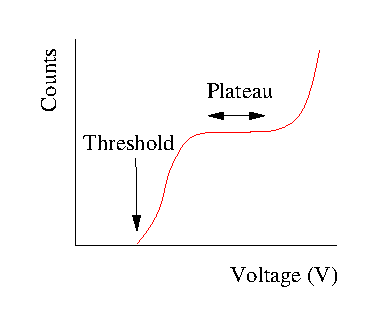
\includegraphics{radiocarbon_dating/geiger1.eps}} \par}
%\vspace{0.3cm}

%(h) Make a plot of counts per minute versus voltage and attach it to your unit.
%Check with your instructor that it looks acceptable.

%\vspace{3.0in}

\textbf{Activity 2: The Properties of Radiation}

An essential attribute of radiation is its ability to penetrate
matter.
Here we will study how three different types of radiation (alpha, beta,
and gamma radiation) penetrate matter. We will do this by using a radiation counter
 and samples of three nuclei.
The heart of the radiation counter is a gas-filled cylinder with a wire at
high voltage running down its center.
This cylinder is called a Geiger-Muller or G-M tube.
Sub-atomic particles flying through the counter ionize atoms in the gas which are 
collected at the center wire producing a voltage pulse that can be measured.
NOTE: Before going any further read the appendix on nuclear safety.

(a) Compare the figure below with your setup. Familiarize yourself with the
different components. DO NOT TOUCH THE FACE OF THE DETECTOR INSIDE
THE SNOUT UNDER ANY CIRCUMSTANCES.

\vspace{0.3cm}
{\centering \resizebox*{0.5\textwidth}{!}{\includegraphics{radiocarbon_dating/rad_counter.eps}} \par}
{\centering Figure 1. Schematic drawing of radiation counter and setup. \par}
\vspace{0.3cm}

(b) Carefully remove the red, plastic cover on the snout of the radiation counter.
DO NOT TOUCH THE FACE OF THE DETECTOR UNDER ANY CIRCUMSTANCES. This would likely
break the window and destroy the counter.

(c) Obtain a set of radioactive sources from your instructor.
Pick one of the sources, place it on the jack, and position the source about 1 cm below
the snout of the radiation counter.
Plug the power cord into a standard electric outlet and make sure the data cable is plugged
into digital channel 1 on the {\it DataStudio} 750 interface.
You should see the power light come on near the base of the counter (which is actually at the
top).
Another light near the snout of the counter blinks whenever a particle
is detected.
If you don't see either light, consult your instructor.

(d) Open the {\it Radiation Counter} activity in the {\bf 132 Workshop} menu and click
the {\bf Start} button on the {\it DataStudio} interface.
Nothing will seem to be happening, but after 30 seconds (watch the clock at the top
of the {\it DataStudio} interface) the number of radioactive decays detected by the 
radiation counter will appear.
Record this result in the appropriate place in the table below.

(e) Now carefully place a piece of plastic on top of the source and run the
counter for another 30 seconds. Record the result below.

(f) Remove the plastic and place a small sheet of lead on top of the source.
Run the counter and record the result.

(g) Repeat steps d-f for the other two radioactive sources.


\vspace{0.3cm}
{\centering \begin{tabular}{|c|c|c|c|}
\hline 
Radiation&
~~~Air~~~~&
~~Plastic~&
~~~Lead~~~\\
\hline
\hline 
\( \gamma \)&
&
&
\\
\hline 
\( \beta \)&
&
&
\\
\hline 
\( \alpha \)&
&
&
\\
\hline
\end{tabular}\par}
\vspace{0.3cm}

(h) Which type of radiation is most penetrating? Why?
\vspace{15mm}

(i) Which type of radiation is least penetrating? Why?
\vspace{15mm}

(j) What material provides the best shielding of radioactivity? Why?
\vspace{15mm}

\textbf{Activity 3: Background Radiation}

(a) Return the radioactive sources to the instructor's table.

(b) With no radioactive sources nearby, make several runs with the radiation counter.
The counts you observe in the detector are due to cosmic rays, radioactive decay
in the building materials surrounding you, and even your own body.
Record the counts and calculate the average and standard deviation of this background
radiation.
\vspace{15mm}

\vspace{1.0in}


\textbf{Activity 4: Nuclear Decay }

To understand the ``clock'' we will use to date the Shroud of Turin we will investigate
how the clock ``ticks''.
In this activity you will use a sample of radioactive material and a nuclear to 
detector to measure the behavior of the material as a function of time.
We will then build a mathematical model of the time dependence of nuclear decay.
We will apply this model to analyze the results of $\rm ^{14}C$ measurements on
the Shroud.

To obtain the radioactive material we will use a procedure known as
``milking the cow''.
We start with a liquid that contains the radioactive isotope $\rm ^{137}Cs$ or
cesium-137.
This isotope decays very slowly; it would take about 30 years for half of a sample
to decay (a bit long for an introductory physics experiment).
However, when $\rm ^{137}Cs$ does decay it usually does so in the following way.

{\centering \( \rm ^{137}Cs \rightarrow e^- + ^{137}Ba(0.662) \) \par}

Notice the additional number ``0.662'' beside the Ba-137. This number means there
is still some energy (0.662 million electron-volts or MeV)
stored in the Ba-137 nucleus and it has not yet reached
its lowest-energy or ground state.
This ``excited'' state of Ba-137 then emits a high-energy photon or gamma ray to 
reach the stable ground state of $\rm {^{137}Ba}$. A diagram of the
process is below. 

\vspace{0.3cm}
{\centering \resizebox*{0.5\textwidth}{!}{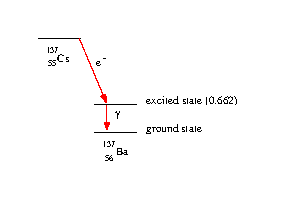
\includegraphics{radiocarbon_dating/Cs-137_decay.eps}} \par}
{\centering Figure 2. Decay scheme of cesium-137. \par}
\vspace{0.3cm}

This intermediate state (labeled ``0.662'') decays quickly to the ground state and
it is the one we will study.

We will prepare a sample of Ba-137 in its excited, 0.662-MeV state 
by starting with a Cs-137 ``generator''.
The Cs-137 produces
Ba-137 at a steady rate. We remove the Ba-137 from the ``generator''
by passing a hydrochloric-acid-saline solution through the generator
(your instructor will do this). This is called eluting which means separate by
washing. The generator is commonly referred to as the ``cow''
and the Ba-137 is ``milked'' from the cow.
The Ba-137 is eluted from the generator and can then be used to study its
decay.


(a) First, make a prediction of the count rate as a function of time.
Sketch your prediction in the space below.

\vspace{1.5in}

(b) What is the mathematical form of your prediction? Why did you choose it?

\vspace{1.5in}

(c) Open the {\it Nuclear Decay} application in the {\bf 132 Workshop} menu. 
When you click {\bf Start}
it will plot the count rate in intervals of 10 seconds.
Get the radioactive sources from your instructor and
try this out with one of them
to make sure you know how to use the hardware and software.
Return the sources to your instructor when you are finished with this test.

(d) Read the rest of this procedure carefully. 
If you have to redo the procedure it may take a long time for the ``generator'' to
produce enough Ba-137 for you to use.

(e) You have a small, metal disk called a planchette that sits on the 
jack which will be positioned close to the snout of the radiation counter.
This will hold the radioactive material.
Put the empty planchette in place and do a ``dry run''.

(f) One team member should be responsible for positioning the planchette.
That person should put on the surgical gloves, eye protection, and a lab coat.
The other team member can run the data acquisition.

(g) When you are ready, alert the instructor. He or she will come over and place 
a few drops of the eluate containing the Ba-137 on the planchette.
Immediately place this under the Geiger counter and
click {\bf Start} on the {\it DataStudio} interface.

{\bf Caution:} Care should be taken in handling the sample.
If any portion of the sample touches your skin immediately wash off in the sink.

(h) Let the data acquisition run for about fifteen minutes or so and then click {\bf Stop}.
Dispose of the planchette according to the guidance from the instructor.

(i) Make a plot of your results using the data in the {\it Counts versus Time Table}. 
Notice that if you 
click on the title of the table, all of the
data will be selected. You can then paste the data into {\it Excel}.
Make sure you subtract the background radiation from your results.

(j) Make a fit to your data. What is the best choice of function for fitting 
your data? How did you make your choice?
Attach a copy of your plot with the fit to this unit.
Record the fit equation below.
Do NOT close your spreadsheet. We may use it later.

\vspace{0.5in}

\textbf{Activity 5: Analyzing Nuclear Decay }

Observation of a sample of radioactive material reveals that the decay
of the atomic nuclei in the sample is determined by statistical processes.
In other words, the number of nuclei N\( _{nuc} \) that decay per
unit time is proportional to the number of nuclei in the sample.

\[
\frac{dN_{nuc}}{dt}\propto N_{nuc}\]


This expression can be turned into an equality by inserting a constant
of proportionality \( \lambda  \) so

\[
\frac{dN_{nuc}}{dt}=-\lambda N_{nuc}\]


where the minus sign is needed because the number of nuclei N\( _{nuc} \)
decreases with time. The decay constant \( \lambda  \) is a characteristic
of each atomic nucleus. 

(a) In the previous activity, you used a particular function to fit 
your data.
Try to prove that you made the right choice by taking derivatives and
seeing if they will satisfy the original differential equation above.
Did it work?
\vspace{30mm}

(b) It is claimed the solution of the differential equation above
describing nuclear decay is the following expression.

\[
N_{nuc}(t)=N_{0}e^{-\lambda t}\]


Prove this statement by taking the derivative of N\( _{nuc} \)(t)
and showing it satisfies the original differential equation. Make
a sketch of the function and describe it in words.
How did your fit function do?
\vspace{40mm}

(c) The decay of atomic nuclei is often characterized by a quantity
known as the half-life \( \tau  \). The half-life is the period of
time for one-half of the original sample to disappear via radioactive
decay. This statement can be expressed mathematically in the following
way.

\[
N_{nuc}(t=\tau )=\frac{N_{0}}{2}\]


Starting with the above expression show that the decay constant \( \lambda  \)
and the half-life are related by the following equation.

\[
\tau =\frac{\ln 2}{\lambda }\]


\vspace{2in}

(d) Now return to the results of your experiment.
Does your count rate fall off exponentially?
Did you fit your data with an exponential? If not,
go back and do so.
Record the decay constant $\lambda$.
\vspace{0.75in}

(e) What is the half-life of Ba-137? Compare this with the accepted value of 2.552 minutes.
\vspace{1.5in}

(f) Consider the following example as a warm-up. A sample of the isotope of iodine
\( ^{131} \)I has an initial decay rate of 1.8 x 10\( ^{5} \) decays/s.
This isotope has a half-life of 8.04 days. It is shipped to a medical
diagnostic laboratory where it will be used as a radioactive tracer.
When the shipment arrives at the lab the decay rate has fallen to
1.4 x 10\( ^{5} \) decays/s. How long did it take for the shipment
to reach the laboratory?
\vspace{2in}


\textbf{Activity 6: Dating the Shroud of Turin }

The previous example shows how one can use the measured decay rate
of an atomic nucleus as a {}``clock'' to determine the passage of
time. The same concept is used in radiocarbon dating. Carbon on the
planet Earth consists largely of three isotopes with A = 12, 13, and
14. The most common form is \( ^{12} \)C and only a very small fraction
of the carbon is \( ^{14} \)C. However, \( ^{14} \)C decays via 

{\centering \( ^{14} \)C \( \rightarrow  \) \( ^{14} \)N + \( \beta ^{-} \)
+ \( \overline{\nu } \)\par}

where \( \beta ^{-} \) is an electron and \( \overline{\nu } \)
is a particle known as a neutrino. Notice this decay does NOT preserve
the number of protons and neutrons in the original nucleus. The ratio
R of \( ^{14} \)C to \( ^{12} \)C on the Earth is 1.30 x 10\( ^{-12} \)
and is roughly constant despite the fact that the \( ^{14} \)C constantly
disappears. The ratio is constant because the supply of \( ^{14} \)C
in the atmosphere is replenished by the reaction of cosmic rays from
outer space with the nitrogen in the upper atmosphere.

Living organisms contain large quantities of carbon and are constantly
exchanging carbon with their surroundings. They contain the same proportion
of \( ^{14} \)C to \( ^{12} \)C as observed in the atmosphere. However,
this proportion begins to change after the organism dies. The \( ^{12} \)C
remains in the dead body, but the \( ^{14} \)C turns into gaseous
\( ^{14} \)N (see decay above) and leaves the body. Hence, the proportion
of \( ^{14} \)C decreases with time, and one has a {}``clock''
that can be used to determine when an organism died. 

The Shroud of Turin is a piece of cloth that bears the image of a
man who appears to have been crucified. It was first displayed in
France in the fourteenth century and has been kept at the Royal Chapel
of Turin Cathedral in a special shrine since 1694. Many believe the
image on the Shroud is of Christ and the cloth is his burial wrap.
In 1989, three laboratories in Arizona in the USA, Oxford in the UK,
and Zurich in Switzerland used advanced methods of radiocarbon dating
in an attempt to determine the age of the Shroud{[}1{]}. The Shroud
is woven of cloth made from plants. Like a living organism that has
died, the \( ^{14} \)C in the Shroud began to gradually disappear
after the plants used to make it were harvested.

(a) The half-life of \( ^{14} \)C is 5730 years. What is the decay
constant \( \lambda  \)?
\vspace{25mm}

\newpage

(b) The three laboratories obtained the following results for the
ratio R of \( ^{14} \)C to \( ^{12} \)C. The ratio of \( ^{14} \)C
to \( ^{12} \)C in the atmosphere is R\( _{i} \) = 1.30 x 10\( ^{-12} \).
What is the implied age of the Shroud for each measurement? Use the
space below for your calculations and enter the results in the table. 

\vspace{0.3cm}
{\centering \begin{tabular}{|c|c|c|}
\hline 
~~~~~Laboratory~~~~~&
~~~~~~~~R\( _{f} \)~~~~~~~~&
~~~~~Age (years)~~~~~\\
\hline
\hline 
Arizona&
1.20 x 10\( ^{-12} \)&
\\
\hline 
Oxford&
1.18 x 10\( ^{-12} \)&
\\
\hline 
Zurich&
1.19 x 10\( ^{-12} \)&
\\
\hline
\end{tabular}\par}
\vspace{0.3cm}

\vspace{5in}
(c) What is the average age of the Shroud? 
\vspace{1in}

(d) The typical uncertainty in these measurements is a standard deviation
of \( \pm  \)40 years. Are the results of the three laboratories
consistent? 
\vspace{1in}

\vspace{15mm}
(e) Is the age of the Shroud consistent with it being the burial wrap
of Christ? 
\vspace{1in}

(f) Are there any reasons to doubt these results?
\vspace{1in}

\textbf{Homework} 

\begin{enumerate}
\item The half-life of a particular radioactive isotope is 6.5 h. If there
are initially 48 x 10\( ^{19} \) atoms of this isotope, how many
atoms of this isotope remain after 26 h? 
\item A radioactive isotope of mercury, \( ^{197} \)Hg, decays into gold,
\( ^{197} \)Au, with a disintegration constant of 0.0108 h\( ^{-1} \).
(a) What is its half-life? (b) What fraction of the original amount
will remain after three half-lives? (c) What fraction will remain
after 10.0 days?
\item The radionuclide \( ^{64} \)Cu has a half-life of 12.7 h. How much
of an initially pure, 5.50-g sample of \( ^{64} \)Cu will decay during
the 2.0-h period beginning 14.0 h later? 
\end{enumerate}

\textbf{The Periodic Chart} 

\begin{center}
%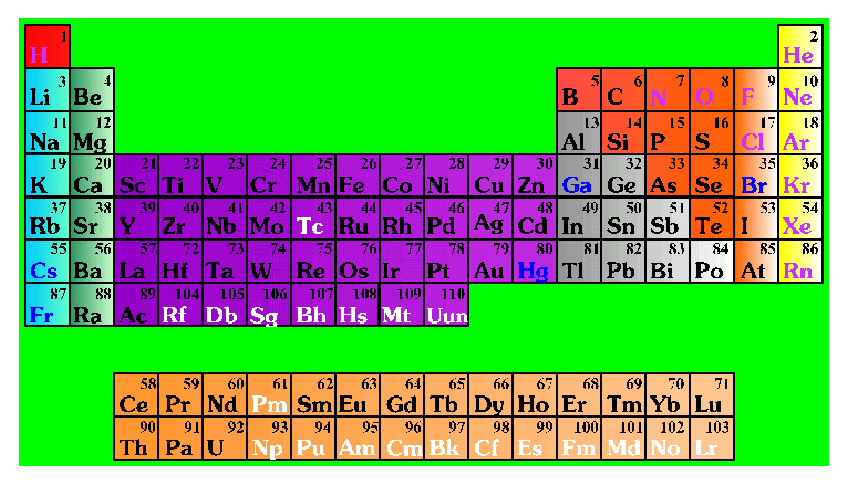
\includegraphics{radiocarbon_dating/pertable2.eps}
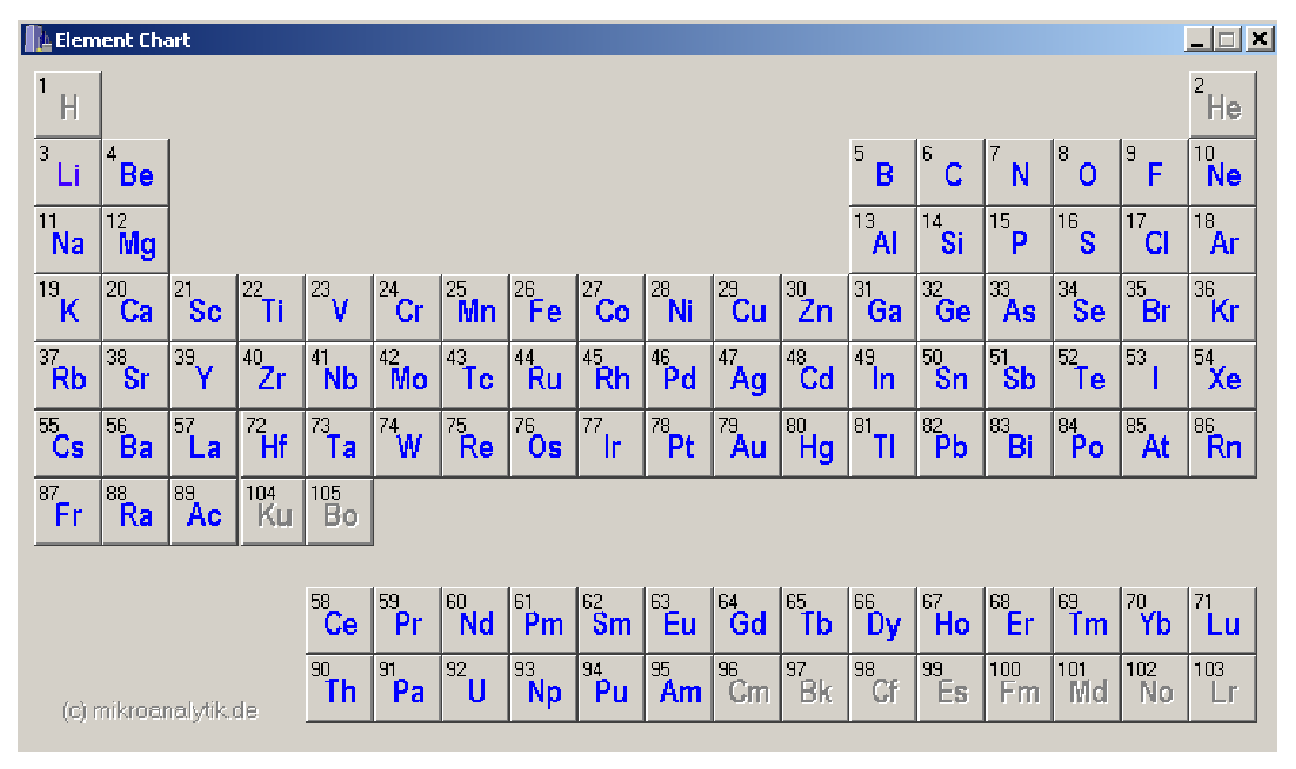
\includegraphics[width=5.5in]{radiocarbon_dating/pertable3.ps}
\end{center}

\textbf{References}

\begin{enumerate}
\item P.E.Damon, D.J.Donahue, B.H.Gore, A.L.Hathaway, A.J.T.Jull, T.W.Linick,
P.J.Sercel, L.J.Toolin, C.R.Bronk, E.T.Hall, R.E.M.Hedges, R.Housley,
I.A.Law, C.Perry, G.Bonani, S.Trumbore, W.Woelfli, J.C.Ambers, S.G.E.Bowman,
M.N.Leese, and M.S.Tite, \emph{Nature}, Vol. \textbf{337}, No. 16,
P. 611-615.\end{enumerate}

